\chapter{Background}
\label{Chapt2}


This chapter will explore the fundamental information relevant to this project, with an emphasis on the world of DNS abuse and transparency. It will include a detailed investigation of the domain name system (DNS), its function in the online community, and the variety of abuses it faces , the history of widely used policies and organisations aimed at mitigating DNS abuse, including a thorough examination of the DNS Abuse Institute and its achievements. A 'competition landscape' providing an examination of current market choices, from automated solutions to human tactics, will be provided as we navigate through the current methodology and technology deployed to mitigate DNS abuse. The reader will obtain a detailed understanding of the current situation of DNS abuse and the need for a more open, strong, and proactive strategy by analysing these various techniques and appreciating their strengths and weaknesses. This chapter emphasises the importance of the suggested solution in an era where digital authenticity is required, not only by providing information, but also by laying the groundwork for its presentation as a better and essential progression in the battle against DNS abuse.

\section{Understanding DNS \& Its Vulnerabilities}

The Domain Name System (DNS) is a significant part of the Internet infrastructure, serving as the key to converting computer-understandable IP addresses into human-friendly domain names. Although the DNS plays a vital role in maintaining ongoing online activities, privacy and security problems still arise. The ScienceDirect paper "Domain Name System Security and Privacy: A Contemporary Survey" provides a detailed analysis of these concerns that highlights the fundamental importance of DNS while illuminating the weaknesses that malicious actors may take advantage of \cite * {Sciencedirect2023dns}. There are a variety of security threats, ranging from DNS infrastructure targeting distributed denial-of-service (DDoS) assaults to cache poisoning and hijacking. Each of these attacks has the potential to do significant harm, including interruptions in service and the promotion of theft and spying. Due to the standard DNS design's lack of encryption, users' query data is vulnerable to abuse and eavesdropping, raising serious privacy problems. However, weaknesses do not mark the end of the story. In the same survey, new approaches are examined to improve DNS security and privacy. The use of DNSSEC (DNS Security Extensions), which authenticates DNS data and guarantees its integrity while repelling some types of attack, is an example of these advances in security measures. In addition, privacy-enhancing technologies are being used to encrypt DNS queries, preventing eavesdropping and manipulation, such as DNS over HTTPS (DoH) and DNS over TLS (DoT). The environment of DNS threats and defences is always changing in sync with the Internet. For systems to be robust and resilient, it is essential to understand these weaknesses and the continuous efforts being made to mitigate them. In this section, we provide an in-depth discussion of DNS vulnerability details, the effects of these safety concerns, and creative solutions that aim to bring in a new era of DNS security and privacy.

In a usual DNS lookup, three types of queries come into play to streamline the process and minimise the data journey. The first type is a recursive query, where the DNS client expects a direct answer or an error if the record cannot be found from the DNS server. Then there is an iterative query, which means if the server doesn't have the answer, it points the client to another server that might know, and the client keeps asking down the line until it gets an answer or hits a dead end. Lastly, a non-recursive query happens when the DNS server already knows the answer either because it is directly responsible for that piece of information or it has it saved from earlier inquiries. This method helps to reduce unnecessary internet traffic and reduce the load on the servers involved.

\section{Strategies \& Collaborations in Addressing DNS Abuse}

The DNS Abuse Institute, which will focus on DNS abuse to help increase safety and security through the domain name system, will be catered on these efforts to address DNS abuse with a comprehensive approach throughout the internet infrastructure. It helps the Internet community identify, report and mitigate DNS abuse in its mission to make the online environment more secure. Efforts by the institute, such as Compass Dashboards, provide vital data to registries and registrars that will enable proper decisions on combating DNS abuse. They show the commitment to transparency and education by issuing publications such as the "DNSAI 2022 Annual Report" or "DNSAI Bulletin 2023 04; Account Takeovers," which provide information on DNS abuse and how recommended mitigation practices \cite{dnsabuseinstitute2023}. Another such global strategy against DNS abuse has been contributed by the Internet Corporation for Assigned Names and Numbers (ICANN)\cite{icann2022dnsabuse} in collaboration with the entire DNS community, ICANN supports a synchronised method in the development of policies and standards on how to mitigate DNS abuse while ensuring the openness of the Internet. These participatory pillars hint at concerted efforts through policy development, technological developments, and stakeholder engagement as a central component in this collective approach to combating DNS abuse \cite{dnsai2022report}. 



\section{Different Forms of DNS Abuse}

DNS abuse takes many forms, each with its procedures and effects on users and the Internet as a whole. It is essential to understand these various pieces of evidence to create responses and regulations that work. This section will examine the comprehensive analysis of DNS abuse presented, describing the description, mechanism, and impact of each kind \cite{dotmagazine2022dnsabuse}.

\subsection{Phishing}
\begin{itemize}
    \item \textbf{Description:} Phishing is a technique aimed at deceiving individuals by creating website addresses that mimic those of companies, to trick users into revealing sensitive information such as login credentials, credit card numbers, or personal identification information \cite{webinarcare2023dnsstats}.
    \item \textbf{Mechanism:} This deception often occurs through emails or messaging services that direct users to websites similar to authentic ones \cite{jakobsson2006phishing}.
    \item \textbf{Impact:} Victims may suffer identity theft, financial fraud, and security compromise.
\end{itemize}

\subsection{Confusable Domains (Typosquatting)}
\begin{itemize}
    \item \textbf{Description:} Registering domain names that look visually similar to popular websites, taking advantage of typing errors or character similarities \cite{inta2023dnstypo}.
    \item \textbf{Mechanism:} Users may accidentally visit these websites when making a typo in a URL, which can expose them to malware or phishing attempts.
    \item \textbf{Impact:} Deception of users and potential harm to brand reputation \cite{edelman2008typosquatting}.
\end{itemize}

\subsection{Domain Hijacking}
\begin{itemize}
    \item \textbf{Description:} Unauthorised acquisition of domain names by exploiting security vulnerabilities in the domain registration system \cite{inta2023dnstypo}.
    \item \textbf{Mechanism:} Attackers may use tactics like social engineering, phishing, or exploiting security loopholes to gain control over a domain.
    \item \textbf{Impact:} Loss of control of the website, redirection to malicious sites, and potential data breaches.
\end{itemize}

\subsection{Botnets}
\begin{itemize}
    \item \textbf{Description:} Botnets involve controlling a group of computers infected with malware, used to carry out attacks or spread spam and malware \cite{citpyour}.
    \item \textbf{Mechanism:} Malware infects computers of unsuspecting users, incorporating them into a network under the attacker's control.
    \item \textbf{Impact:} Can result in large-scale DDoS attacks, mass spam campaigns, and widespread malware dissemination.
\end{itemize}

\subsection{Fast Flux Hosting}
\begin{itemize}
    \item \textbf{Description:} A technique used to conceal the location of websites associated with phishing and malware distribution \cite{lin2013genetic}.
    \item \textbf{Mechanism:} Involves a network of compromised hosts that regularly modify DNS records to avoid detection.
    \item \textbf{Impact:} Makes tracking and shutting down malicious sites difficult.
\end{itemize}

\subsection{Domain Generation Algorithms (DGA)}
\begin{itemize}
    \item \textbf{Description:} DGAs generate domain names that act as meeting points for botnets \cite{antonakakis2012throw}.
    \item \textbf{Mechanism:} Malicious software uses algorithms to generate a sequence of domain names for command-and-control servers.
    \item \textbf{Impact:} Adds complexity to efforts to disrupt botnet command and control channels.
\end{itemize}

    
\subsection{Dangling DNS Records}
\begin{itemize}
    \item \textbf{Description:} Dangling DNS record means a DNS entry pointing to a resource (like around an IP address or domain name) that is under the control of the owner of the originating domain. This occurs in a scenario where cloud resources are being decommissioned and the respective DNS records for such resources are not updated \cite{friess2024cloudy}.
    \item \textbf{Mechanism:} These unclaimed DNS entries will then become available for any attacker to set up malicious services on those resources, effectively "hacking" the traffic intended for the services from the original domain.
    \item \textbf{Impact:} The impacts of the exploitation can result in some security issues, such as phishing, malware distribution, and data intercepting, which puts end-user information at risk from other cybercrime activities against them and their organisation.
\end{itemize}


\captionsetup{font= footnotesize}
\begin{figure}[H]
\centering
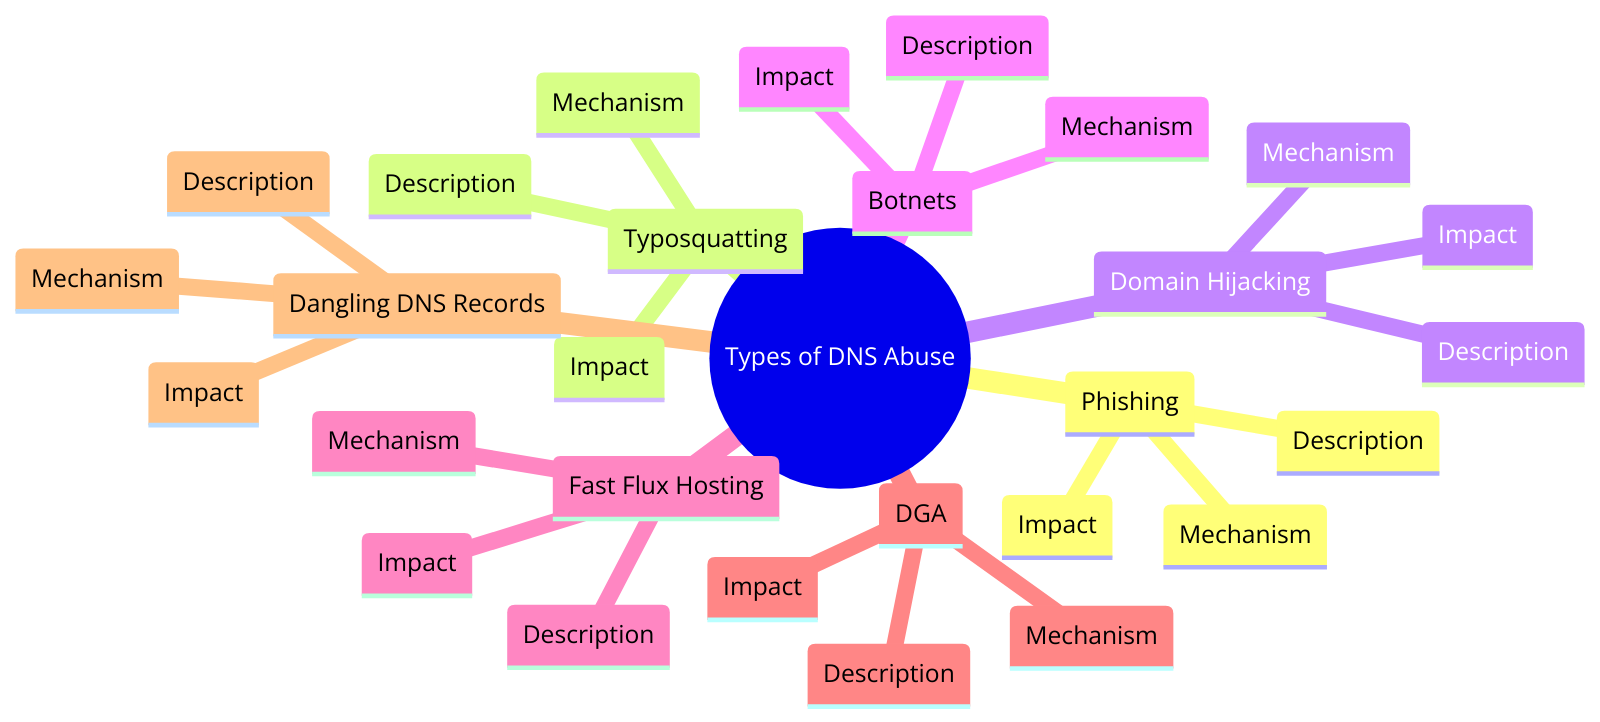
\includegraphics[width=\textwidth]{background/dnsformstypes.png}
\caption{Different Forms of DNS Abuse.}
\label{fig:figureThree}
\end{figure}




\section{How DNS Abuse Harms Users}

DNS abuse has serious and detrimental effects for both users and organisations, going beyond basic technological disruptions. Identity theft is among the most direct and direct effects. Phishing attacks, a common type of DNS abuse, use realistic websites to trick visitors into revealing sensitive data. Such attacks can produce information that results in financial theft, unauthorised access to accounts, and long-term damage to a person's reputation and credit \cite{godaddy2023dnsabuse}.

\subsection{Identity Theft}
\begin{itemize}
    \item \textbf{Phishing:} Phishing attacks often use domain names that imitate legitimate websites, fooling users into providing sensitive information such as usernames, passwords, or financial details, leading to potential identity theft.
\end{itemize}

\subsection{Financial Loss}
\begin{itemize}
    \item \textbf{Deceptive Transactions:} Users may be tricked into making payments to deceptive websites or unknowingly disclose their credit card information, resulting in financial losses \cite{bohme2013economics}.
\end{itemize}

\subsection{Data Breach}
\begin{itemize}
    \item \textbf{Malware:} Malicious software spread through compromised DNS systems can allow unauthorised access to corporate data, leading to data breaches \cite{fowler2016data}.
\end{itemize}

\subsection{System Compromise}
\begin{itemize}
    \item \textbf{Malware Infection:} Systems infected with malware due to DNS abuse can be exploited for further attacks, including the creation of botnets or the distribution of ransomware, resulting in system compromise \cite{saxe2018malware}.
\end{itemize}
\captionsetup{font= footnotesize}
\begin{figure}[H]
\centering
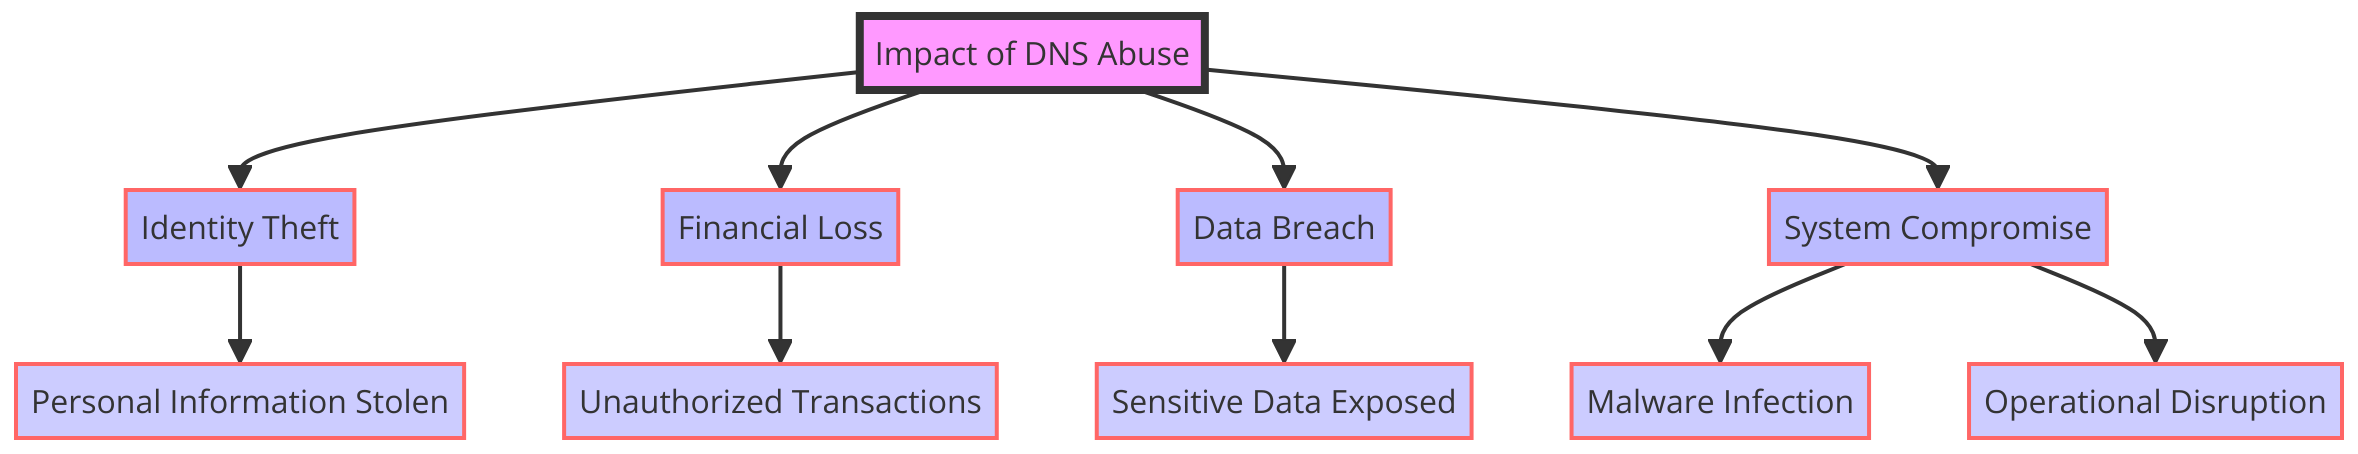
\includegraphics[width=\textwidth]{background/DNSabuseHarm.png}
\caption{How DNS Abuse Harms Users.}
\label{fig:figureFour}
\end{figure}


\section{Future Dangers of DNS Abuse}

As technology develops, so do bad actor strategies and tools, creating a dynamic environment for DNS abuse that could present new risks in the future. The sophistication of attacks has increased, which is a major issue. Bad actors are always creating increasingly sophisticated methods to take advantage of DNS, such as creating more convincing phishing schemes and using advanced virus distribution networks \cite{icann2022dnsabusetrends}.

\subsection{Increased Sophistication}
\begin{itemize}
    \item \textbf{Evolving Techniques:} Bad actors are constantly developing more sophisticated techniques to exploit DNS, such as advanced phishing schemes and malware distribution \cite{wrightson2014advanced}.
\end{itemize}

\subsection{IoT Vulnerabilities}
\begin{itemize}
    \item \textbf{Expanding Vulnerabilities:} The widespread adoption of Internet of Things (IoT) devices, which often lack robust security measures, presents a growing target for DNS-based attacks \cite{mahmoud2015internet}.
\end{itemize}

\subsection{Infrastructure Attacks}
\begin{itemize}
    \item \textbf{DNS as a Prime Target:} Attacks on DNS infrastructure can disrupt internet services on a large scale, including DDoS attacks targeting DNS providers or exploiting weaknesses in DNS protocols \cite{dooley2017dns}.
\end{itemize}

\subsection{Deepfakes \& AI}
\begin{itemize}
    \item \textbf{AI-Enhanced Phishing:} The use of AI technologies, such as deepfakes, has made phishing attacks more convincing and deceptive, manipulating audio and video content to impersonate trusted entities \cite{schick2020deep}.
\end{itemize}

\subsection{Cloud Computing Vulnerabilities}
\begin{itemize}
    \item \textbf{Targeting Cloud Services:} As organisations increasingly rely on cloud-based services, bad actors are exploiting DNS vulnerabilities to attack these platforms, potentially leading to data breaches and service disruptions \cite{mather2009cloud}.
\end{itemize}

\subsection{Mobile Device Exploitation}
\begin{itemize}
    \item \textbf{Mobile DNS Attacks:} The rising usage of mobile devices has led bad actors to target smartphones and tablets through DNS-based attacks, which can lead to data theft and the spread of malware \cite{au2016mobile}.
\end{itemize}

\subsection{Cryptocurrency \& Blockchain Exploitation}
\begin{itemize}
    \item \textbf{Crypto-Related DNS Attacks:} Attackers could exploit DNS vulnerabilities to redirect users to fake cryptocurrency exchanges or blockchain platforms, leading to financial fraud and theft of digital assets \cite{bashir2019advanced}.
\end{itemize}

\subsection{Political and Information Warfare}
\begin{itemize}
    \item \textbf{DNS in Cyber Warfare:} The manipulation of domain name systems can be used to spread misinformation or disrupt services during significant political events, serving as a tool for political and information warfare \cite{chapple2021cyberwarfare}.
\end{itemize}

\subsection{Exploiting Emerging Technologies}
\begin{itemize}
    \item \textbf{Abuse in New Tech Domains:} As new technologies such as 5G, AI, and quantum computing advance, tactics involving DNS abuse are likely to evolve, potentially leading to more sophisticated attacks \cite{brunner2021cybersecurity}.
\end{itemize}

\subsection{Supply Chain Attacks}
\begin{itemize}
    \item \textbf{DNS in Supply Chain Compromise:} DNS manipulation can also be employed as part of supply chain attacks, targeting software updates or cloud-based services to compromise organisations \cite{boyson2014cyber}.
\end{itemize}



\captionsetup{font= footnotesize} 
\begin{figure}  [H]
    \centering
    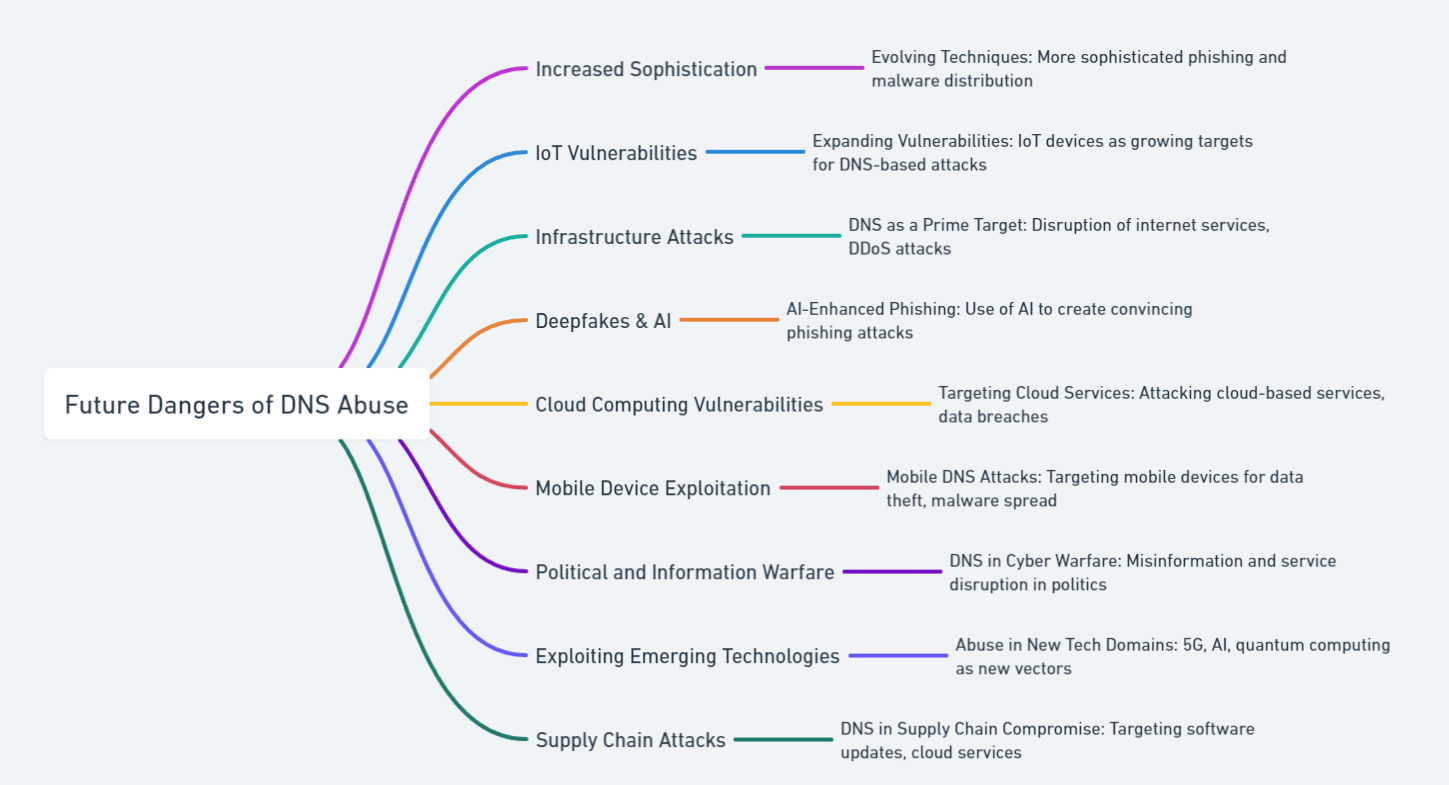
\includegraphics[width=\textwidth]{background/Future Dangers of DNS Abuse.png}
    \caption{Future Dangers of DNS Abuse.}
    \label{fig:LOLOLOL}
\end{figure}

By understanding these future dangers and emerging trends, stakeholders can better prepare and adapt their strategies to anticipate and counteract the evolving nature of DNS abuse.


\section{Foundational Mitigation Strategies \& Best Practices }

To address the broad nature of threats, mitigating DNS abuse requires an integrated strategy that integrates multiple strategies and best practices. The establishment of reporting and monitoring procedures is one fundamental tactic. Automated systems have the ability to track domain name registration patterns that may indicate DNS abuse, and protocols to report questionable actions can help ensure prompt intervention \cite{icannndnssec}. To confirm security and ensure that systems have not been compromised, regular audits of DNS configurations and domain registrations are also necessary \cite{lucas2021tls} .

\begin{enumerate}
    \item \textbf{Monitoring \& Reporting}
    \begin{itemize}
        \item Implementation: Use automated systems to monitor domain name registration for patterns that may indicate DNS abuse \cite{icannndnssec}. Establish procedures for reporting activities to authorities or cybersecurity organisations \cite{lucas2021tls}.
    \end{itemize}
    \item \textbf{Security Awareness Training}
    \begin{itemize}
        \item Implementation: Develop training programmes for users and IT staff with a focus on recognising phishing attempts, practising browsing habits, and understanding DNS security.
    \end{itemize}
    \item \textbf{DNS Security Extensions (DNSSEC)}
    \begin{itemize}
        \item Implementation: Deploy DNSSEC to ensure the integrity of the DNS data. This involves signing DNS records to protect against modification and DNS spoofing.
    \end{itemize}
    \item \textbf{Multi-Factor Authentication (MFA)}
    \begin{itemize}
        \item Implementation: Enforce multifactor authentication (MFA) for domain registrars and interfaces used to manage DNS \cite{icannndnssec}. This adds a layer of security beyond passwords, helping to prevent unauthorised domain transfers or alterations \cite{moghaddam2014ecco}.
    \end{itemize}
    \item \textbf{Blacklisting \& Takedown Services}
    \begin{itemize}
        \item Implementation: Collaborate with cybersecurity firms to identify and blacklist domains engaged in malicious activities. Establish response teams dedicated to removing domains involved in DNS abuse.
    \end{itemize}
    \item \textbf{Collaboration}
    \begin{itemize}
        \item Implementation: Foster collaboration among Internet service providers (ISPs), domain registrars, governments, and cybersecurity organisations. Share intelligence and best practices to collectively improve defence against DNS abuse \cite{skopik2017collaborative}.
    \end{itemize}
    \item \textbf{Regular Audits}
    \begin{itemize}
        \item Implementation: Conduct security audits of domain registrations and DNS configurations to verify their security and ensure that they have not been compromised \cite{coronado2014auditing}.
    \end{itemize}
    \item \textbf{Machine Learning}
    \begin{itemize}
        \item Implementation: Using AI and machine learning algorithms to analyse patterns in DNS traffic and proactively predict instances of DNS abuse \cite{icannndnssec}. This proactive approach enables the identification of threats before they materialise \cite{tsukerman2019machine}.
    \end{itemize}
    \item \textbf{Geo-Blocking \& IP Filtering}
    \begin{itemize}
        \item Implementation: Deploy geo-blocking and IP filtering techniques to limit access to DNS services from regions that have a history of DNS abuse. This can reduce the risk that attackers will use these services to carry out malicious activities or distribute malware \cite{meeseedited}.
    \end{itemize}
    \item \textbf{Enhanced Domain Validation Procedures}
    \begin{itemize}
        \item Implementation: Enhance the domain registration process by implementing validation procedures. This may involve verifying the identity of individuals or organisations that register domains, especially domains that resemble brands or fall into sensitive categories. By taking these measures, we can strengthen security and mitigate the risks associated with fraudulent domain registrations.
    \end{itemize}
\end{enumerate}


\captionsetup{font= footnotesize}
\begin{figure} [H]
    \centering
   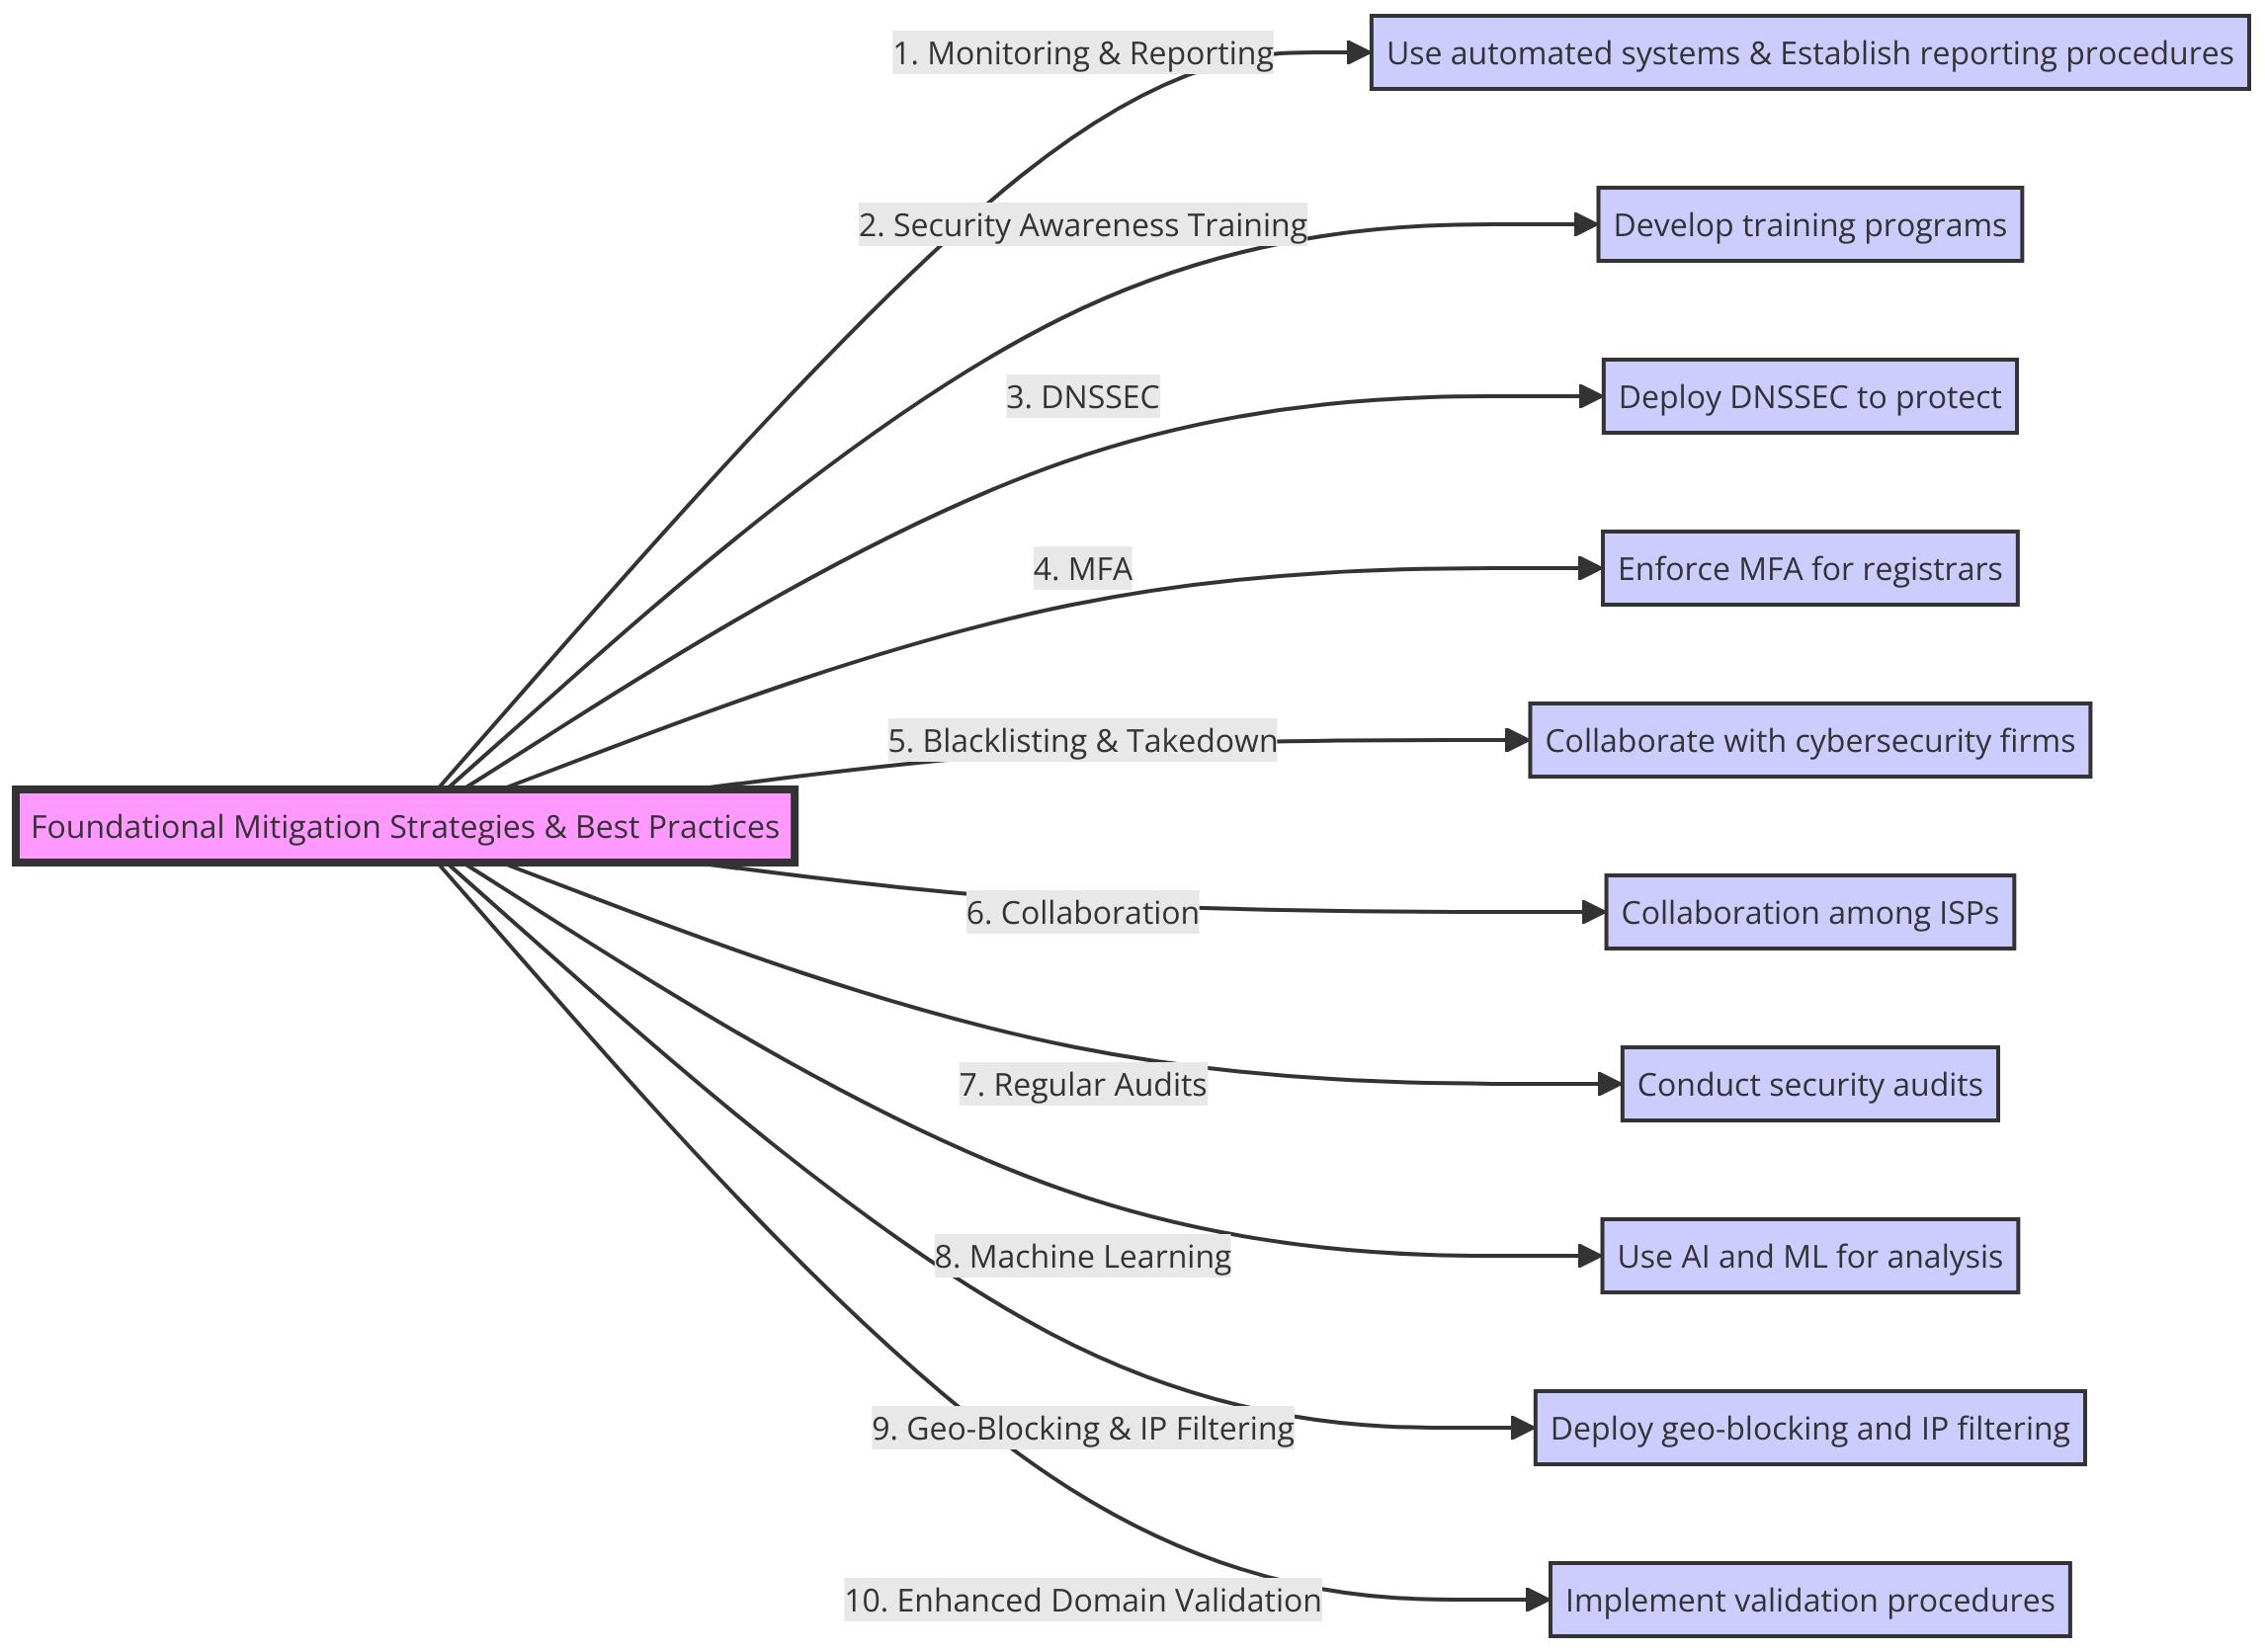
\includegraphics[width=1.1\textwidth]{background/diagram (7).png}
    \caption{Mitigation Strategie.}
    \label{sadasdasdada}
\end{figure}

Each of these strategies plays a role in creating a comprehensive defence against DNS abuse. By integrating these tactics, organisations can establish robust, proactive measures to detect, prevent, and mitigate the ever-evolving threats posed by DNS abuse.

\section{Summary \& Synthesis}

After exploring the different forms of DNS abuse , How DNS abuse harms the user, Future Dangers of DNS abuse, and Mitigation Strategies and Best Practices. I have designed a table that has DNS abuses and the best possible mitigation strategies to help them against them, taking into account the transparency story behind it , user harm and reasoning. 


{

\footnotesize

\begin{longtable}{|p{2.5cm}|p{2.5cm}|p{4cm}|p{3cm}|p{4cm}|} 

\hline
\cellcolor{gray!50}\textbf{DNS Abuse } & 
\cellcolor{gray!50}\textbf{User Harm} & 
\cellcolor{gray!50}\textbf{Mitigation Strategy} & 
\cellcolor{gray!50}\textbf{Reasoning} & 
\cellcolor{gray!50}\textbf{Transparency Aspect} \\ \hline
\endfirsthead

\multicolumn{5}{c}%
{
\hline \cellcolor{gray!50}\textbf{DNS Abuse} & 
\cellcolor{gray!50}\textbf{User Harm} & 
\cellcolor{gray!50}\textbf{Mitigation Strategy} & 
\cellcolor{gray!50}\textbf{Reasoning} & \cellcolor{gray!50}
\textbf{Transparency Aspect} \\ \hline
\endhead

\hline \multicolumn{5}{|r|}{{\cellcolor{gray!50} Continued on next page}} \\ \hline
\endfoot

\hline
\endlastfoot
Phishing & \mbox{Identity Theft}, Financial Loss &  \mbox{Security Awareness} \mbox{Training, Enhanced Domain} Validation Procedures & \mbox{Training helps users} \mbox{recognize phishing} \mbox{attempts. Validation} prevents the registration of mimic domains. & \mbox{Increases awareness and} \mbox{scrutiny during domain} registration. \\ \hline

\mbox{Confusable} Domains \mbox{(Typosquatting)} & Unauthorised Account Access & \mbox{Enhanced Domain} \mbox{Validation Procedures}, Regular Audits & \mbox{Prevents Registration} of Similar Domains. \mbox{Audits ensure} \mbox{compliance.} & \mbox{transparent domain} \mbox{registration process.} \\ \hline

\mbox{Domain} \mbox{Hijacking} & \mbox{System} \mbox{Compromise}, \mbox{Data Breach} & \mbox{Multi-Factor Authentication} (MFA), Regular Audits & \mbox{MFA secures domain} management. \mbox{Audits verify security} measures. & \mbox{Accountability in domain} management. \\ \hline

Botnets & \mbox{Malware} \mbox{Distribution} & Collaboration,Machine Learning & \mbox{Intelligence Sharing} \mbox{identifies botnet} \mbox{activities. AI predicts} \mbox{the formation of} \mbox{botnets}. & \mbox{Shared responsibility and} proactive detection. \\ \hline

\mbox{Fast Flux} \mbox{Hosting} & \mbox{System Infections} & Blacklisting and Takedown Services, Geo-Blocking & \mbox{Rapid response to} \mbox{malicious domains.} restrict access from risky regions. & Responsive and transparent threat management. \\ \hline

\mbox{Domain} \mbox{Generation} Algorithms (DGA) & \mbox{Malware} \mbox{Distribution} & \mbox{Machine Learning, DNS} \mbox{Security Extensions} (DNSSEC) & AI detects abnormal \mbox{patterns. DNSSEC} \mbox{prevents spoofing.} & Integrity and trust in DNS data. \\ \hline

\mbox{Dangling DNS} Records & Service Disruption & Monitoring and Auditing of DNS Records & \mbox{Regular monitoring} \mbox{allows for the early} \mbox{detection of dangling} \mbox{DNS records,} \mbox{reducing the window } \mbox{of opportunity for} attackers. & Promotes proactive security \mbox{practices and reduces} \mbox{the incidence of service} interruptions \\ \hline

\mbox{IoT} \mbox{Vulnerabilities} & \mbox{Unauthorised} \mbox{Access, Data} \mbox{Breach} & \mbox{Security Awareness} \mbox{Training, Collaboration} & \mbox{Educates on security} \mbox{practices.} \mbox{Collaboration on best} \mbox{practices.} & \mbox{Open exchange of} \mbox{knowledge and efforts.} \\ \hline

Infrastructure Attacks & \mbox{DDoS Attacks}, \mbox{System Downtime} & DNSSEC, Collaboration & Protects DNS Data Integrity. Sharing of threat intelligence. & \mbox{Collective action}  \mbox{strengthens the DNS} infrastructure.  \\ \hline

Deepfakes and AI & \mbox{Identity Theft}, \mbox{Misinformation} & \mbox{Security Awareness} \mbox{Training, Monitoring} & \mbox{Recognising Phishing.} \mbox{Monitor} \mbox{AI threats.} & \mbox{Vigilance and prompt} \mbox{threat reporting.} \\  \hline

\mbox{Cloud} \mbox{Computing} Vulnerabilities & \mbox{Data Breach}, \mbox{Unauthorised} Access & Regular Audits, Enhanced Validation & \mbox{Secure DNS settings} \mbox{in cloud services.} \mbox{Prevents exploitation.} & \mbox{Framework for secure} \mbox{domain use in cloud.} \hline

\mbox{Mobile Device} Exploitation & Unauthorised Access, Financial Loss & \mbox{MFA, Security Awareness} Training & \mbox{Secures account} \mbox{access.} \mbox{ Raises awareness} of threats. & Mobile security awareness and protection. \\ \hline

\mbox{Political and} Information Warfare & Misinformation, Political \mbox{Manipulation} & Monitoring, Collaboration & \mbox{Monitoring abuse in} \mbox{campaigns. Unified} \mbox{response to } \mbox{misinformation.} & Transparency in monitoring and collective action. \\ \hline

\mbox{Exploiting} Emerging \mbox{Technologies} & system \mbox{Vulnerabilities} &\mbox{ Machine Learning,} \mbox{Collaboration} & \mbox{Analytics to predict} \mbox{DNS abuse. Share} \mbox{knowledge about} \mbox{threats.} & \mbox{Innovation in defense}  \mbox{strategies and sharing.} \\ \hline

\mbox{Supply Chain} \mbox{Attacks} & \mbox{System} \mbox{Compromise,} Data Breach & Regular Audits, Blacklisting & \mbox{Audits for DNS} \mbox{integrity. Rapid} \mbox{response to threats.} & \mbox{Transparency in supply} \mbox{chain security.} \\ \hline

\caption{Mitigation strategies against DNS abuse and its impact on users.} 

\end{longtable}

}


Finally, this chapter has examined all aspects of DNS abuse,  the various forms, the serious harm it does, and potential future threats. Understanding these ranges and the effects they can have is important for the development of regulation and measures. Both the DNS Abuse Institute and ICANN have taken great steps in dealing with this issue. With the advancement of technology and the growing threats, it is more of an adaptive and collaborative approach that remains the key. Possible mitigation techniques that have been discussed outline a guide to the possible approach to combating DNS abuse such as advanced technology, enhanced validation, and continuous monitoring. Cooperation with the use of new technologies is indicated, hence, in DNS abuse mitigation, to reach a joint effort in the management of abuse. Thus, a comprehensive strategy would, of course, call for some appropriate tools, but it would also be a combination of approaches and, most importantly, cooperation from the industry. The evolution of the digital landscape requires adaptable approaches to maintain the security of the DNS and Internet infrastructure.

By understanding the connections between different aspects of DNS abuse and reinforcing the collective effort required for effective mitigation, stakeholders can be better prepared to face the challenges ahead. This chapter sets the stage for further research and action, with the aim of contributing to a safer and more secure digital world.



\chapter{State of the Art}

This chapter explores the strategies used to mitigate DNS abuse and new developments in this field. Explore and evaluate the effectiveness and transparency of multiple mitigation techniques, including DNS filtering and threat intelligence, in which experts organise and analyse information about cyber attacks. Additionally, the use of domain-generating techniques and DoT and DoH are two novel forms of DNS abuse that are highlighted in this section. In addition, the role of AI and machine learning in identifying and mitigating DNS abuse is covered. The final half of the section includes a discussion on potential future research areas and technologies to improve DNS abuse mitigation. Case studies offer practical information on DNS abuse occurrences. 


\section{Current Strategies and Their Effectiveness in Relation to DNS Abuse}


DNS abuse presents a significant challenge for Internet entities involved in domain name management. Various approaches are employed to mitigate such abuse, including DNS filtering, which regulates access to specific websites and prevents you from accessing malicious sites that can administer phishing and ransomware. Additionally, threat intelligence methodologies use data analysis to identify potential risks, as exemplified by \cite{schmid2021thirty}. Anomaly detection plays a role in identifying suspicious DNS activities indicative of malicious intent using Packet Analysis to analyse individual packets for DNS allowing for real-time detection and statistical analysis, which involves performing statistical analysis on a large dataset of DNS traffic. However, these methods can face operational challenges, such as errors and the need for fast access to critical threat data. 

\subsection{Transparency in DNS Abuse Mitigation \& DNS Relevance}

\begin{enumerate}
    \item A Case Study of Cloudflare's Transparency Approach



Cloudflare is committed to maintaining transparency \cite{cloudflare_transparency_2022}, which is the keystone of their relationship with customers, guiding each of these approaches to reports of abuse of the DNS and requests that may come from law enforcement. All of these reduce their actions and policies in moulding a trustworthy environment in light of addressing Internet safety and privacy concerns. Their approach to handling DNS abuse reports and law enforcement requests is anchored on three core principles:


\begin{enumerate}
    \item Require due process: Cloudflare will comply with due process as required by law, remaining neutral and not exceeding legal requirements.
    
    \item Respect privacy: Cloudflare respects your privacy and will never sell or otherwise share any personal or private information with any third party without your explicit permission. This is applicable to each and every request.
    
    \item Provide Notice: Cloudflare will notify customers if legal requests are made for their information, unless prohibited by law.

\end{enumerate}

The Cloudflare Transparency Report gives deep statistics and trends based on DNS abuse reports on Cloudflare's response: 

\begin{enumerate}
    \item Abuse Reports: Cloudflare actively responds to abuse reports, including phishing, malware, and copyright infringement.

    \item Actions taken: Cloudflare may terminate services for domains involved in abuses such as phishing or malicious activities.
    
    \item Termination of services: 206 accounts and 530 domains are suspended for the latter half of 2022 for hosting domains associated with CSAM that were not compliant with reported issues.
    
    \item UDRP Requests: Cloudflare responded to 21 UDRP (Uniform Domain Name Dispute Resolution Policy) requests from an ICANN-approved dispute board in the second half of 2022.
    
\end{enumerate}

In addition , Cloudflare's careful description of compliance and due process with respect to handling law enforcement requests comes from their latest Transparency Report. Below is a summary of the major areas covered.

\begin{enumerate}
    \item Legal Sufficiency Review: Cloudflare reviews the legal validity of requests before taking any action according to the law and respects the privacy of the users. Cloudflare responds only to valid law enforcement requests, including court orders and subpoenas.

 \item Respect to International Privacy Laws: Cloudflare checks the disparity of the request, rejecting to honour it if it is at odds with the rights enshrined by the privacy laws of the two countries.


 \item Emergency disclosure requests: Cloudflare only considers making emergency disclosures to law enforcement where there is an imminent danger of harm and clearly requires a stated intention for the follow-up of legal processes.

 \item  National Security Requests and Non-Disclosure Obligations: National security orders are incompatible with the company's aims of transparency; thus, Cloudflare is challenging them.

 \item  International Requests for Data: Cloudflare reviews such requests from the foreign government in accordance with the United States legal process or on a case-by-case basis consistent with international norms and policies.

\end{enumerate}

Public reporting by Cloudflare and working closely with law enforcement, as well as other partners, form important elements in its strategy of mitigating DNS abuse such as: 

\begin{enumerate}

\item Reporting to the Public \& Transparency: Cloudflare opens its data to the public to showcase the types and the volume of abuse reports for trust-building and to exemplify the notion of efforts against antiabuse.

\item Law Enforcement Cooperation: Cloudflare partners with law enforcement regarding the privacy of citizens in such a way that it makes sure the proper legal justification of the actions in relation to DNS abuse.


\item Mitigation actions: Cloudflare makes a proactive effort to prevent DNS abuse by stopping access to any offending domains that are used in phishing, malware distribution, and other damaging activities.

\item Challenges to Mitigating DNS abuse: Cloudflare admits to striking a balance between free speech, legal matters, and the need for stakeholders' joint efforts in the quest to fight DNS abuse.

\item Efficiency of Efforts to Mitigate DNS Abuse: Although successful mitigation involves tackling the root causes and diversity within the market, Cloudflare's transparency reports help in understanding abuse mitigation efficiency.

\end{enumerate}

Some of the challenges the Transparency Report showcases that Cloudflare is grappling with the complexity of DNS abuse, how to achieve a balance between transparency and privacy, and being legally and regulatory compliant, besides also having technical limitations in the mitigation of misuse. This allows ideas to be used to improve processes.

\begin{enumerate}
    \item Enhanced Cooperation with Stakeholders: Cloudflare proposes that such a relationship with law enforcement, service providers, and international organisations will be an industry best practice to standard procedures to increase the efficacy of the internet by mitigating DNS abuse.
    
    \item Improve Abuse Detection Systems: Cloudflare said it would invest its capital in funding more development in advanced technologies, machine learning, and further enhancement of abuse detection systems to allow for faster identification and mitigation of abusive content.
    
    \item Transparency Reporting Enhanced: Cloudflare looks forward to providing even more granular transparency reports that would give deep insight into the types of abuse on DNS and the effectiveness of its mitigation for improved abuse handling practice.

    \item Better User Education \& Awareness: The focus is to develop more educational materials and programmes to inform the user, bringing to their notice the risks of cybersecurity and DNS abuse for a safer Internet environment.

    \item Advocate Policy and Legal Reforms: Cloudflare works to propose and advocate policy and legal reforms, which could be embraced in mitigating any potential collision points between privacy laws and law enforcement requests, hence balancing user privacy with the fight against DNS abuse.
    
    \item Create a Multi-stakeholder Feedback Mechanism: A mechanism can be put in place that ensures feedback not only from the users but also from the civil society and other stakeholders; that would bring out to what extent Cloudflare was able to be successful in their efforts towards transparency and reduction of abuse. Such recommendations can be useful for guiding any further policy-making or organisational policy enhancements.
    

\end{enumerate}

In conclusion, the company emphasises its commitment to protecting legal processes and user privacy while navigating government and law enforcement requests. A critical aspect of these reports is Cloudflare's approach to DNS requests, particularly regarding content blocking through its 1.1.1.1 Public DNS Resolver.This was the key answer: Cloudflare, in no uncertain terms, "received legal requests to block content at our DNS servers" and stated its policy to first "exhaust legal remedies" that they could enforce. This is an indication of how very carefully Cloudflare has to adhere to the demands of the law, yet protect the openness of the Internet, bringing out just how major DNS is in all matters that pertain to the accessibility of content on the Internet and governance of the Internet.

\item Google Transparency Reports 

This shows the weight attached to the Domain Name System (DNS) when enforcing the requests from the global governments, more so in between them and the internet governance, in relation to the content removal from Google services. Data from Russia, with tens of thousands of redaction requests, might signal broader actions that include DNS-level interventions. This highlights the kind of role DNS plays in controlling access to the Internet or blocking content, which is usually put under legal and regulatory pressures from major tech companies, including Google.

Any question related to these requests, although not directly related to the manipulation of DNS, implies the possibility of any technical adjustment to be carried out in order to fulfil the criteria directly affecting DNS resolutions. This indirect reference considers DNS to be one of the critical infrastructures in the debate on Internet governance, censorship, and access to information. What it does is show the Google Transparency Report, which indicates the fact that DNS is an important architecture of the Internet and is also a trouble spot for exercising control over digital content and information flow \cite{Google2023}.

\item Amazon Transparency Reports 

Necessarily, such a role of DNS in servicing governments or other legal data demands does not trace directly to specific acts of manipulation in the DNS or intervention at the domain-level. The report explains about Amazon's observance of due process laws in handling requests for data such as subpoenas and search warrants, with a lot of emphasis on customer privacy and protection of data which can be mounted against the state or any other third party institution or person. It goes without saying that handling the domain or the services to do with this website means that a possibility of such a move as DNS changes can be in the offing. However, they do not give clear examples where DNS interventions have been taken, but describe the circumstances related to legal compliance and internet governance without direct reference to DNS \cite{Amazon2023}.

\item The CyberGhost Transparency Report

An obvious upward trend of the recursion without DMCA complaints, along with flagging malicious activities, flashes up in each year, record by record, before a sudden spike around 2023. Given the growing level of claims and requests, CyberGhost still regards the No Logs policy as a strong sweat so they keep a keen eye and hence stays guardedly strong on the user's privacy and any request relating to DNS. The report is categorical with such an idea that even in the case of mitigating malicious activity, they do not involve logging of DNS queries or respective user activity; therein, the integrity of user data and an assurance towards compliance in privacy. DNS somehow plays a function in this case: It becomes evident that the design of the CyberGhost infrastructure is supposed to be resistant to infiltrators and, hence, capable of withstanding invasions and pressures in no less than those that would compromise an individual's anonymity and right to freely receive information via the Internet \cite{CyberGhostVPN2023}.

\item The Meta-Transparency Reports

At the same level of social media, the enforcement of intellectual property rights, including Facebook and Instagram, shall entail the enforcement of a comprehensive strategy targeting copyright, counterfeit, and trademark infringements, with an important focus on the Domain Name System (DNS) as the centre stage for such activities. The DNS serves both as a foundation for the distribution of information on-line and as a checkpoint in the enforcement process. For example, content removals from Facebook and Instagram amount to 447,123 and 297,356, respectively, in the first half of 2022. This shows a scenario in which interventions range from more than platform moderation to include DNS-level actions of deindexing websites or altering DNS records to block access to infringing content.

The sustained rate of content removals since the latter halves of 2020 and 2021 indicates a reliance on DNS mechanisms. This may explain the huge year-over-year drop in Facebook's copyright and counterfeit content takedown requests from 2020-2021. It would seem that Meta (the parent company of Facebook) may not work with DNS providers to have the offending domains taken down, but instead remove the infringing content. This underscores how important DNS is in the enforcement of intellectual property rights, the checks on the spread of the counterfeit, fake, and grey markets, and in protecting the rights of the owner of intellectual property and trademarks  \cite{Facebook2023}.

\item  T-Mobile Transparency Report

It outlines how the company complies with directions of the law in the management of requests for information from consumers, thus highlighting staying within customers' privacy and legal compliance. Details the approach and policies of the company in response to lawful requests on records of customers within T-Mobile, Metro by T-Mobile, and Sprint, now collectively T-Mobile USA, Inc. (TMUS). At the same time, it provides information about what TMUS does to protect consumers from unauthorised data access, including first-party requests made by the company itself, such as subpoenas, court orders, and warrants, with all processes required following the same. When sharing details surrounding the number and types of requests received in 2022, the report marks a heavy emphasis on TMUS’s efforts to take care of customer privacy and complying with applicable legal obligations. In the case of T-Mobile, it handled 301,388 subpoenas, mostly related to orders to disclose information about the subscriber, such as names and addresses, and 94,599 different types of warrants or search warrants, which can be after historical location data or the content of messages \cite{TMobile2022TransparencyReport}.

\item IBM 1H 2021 Law Enforcement Requests Transparency Report
 
 IBM focuses on data ethics and transparency, just as it has done throughout the years to build trust among clients. The emphasis is on who owns the data and promotes client data policies, belonging to the government, and being fair and not discriminatory. The IBM report aims to make it clear where the company stands on the issue of client data that go through government surveillance. Therefore, it advocated that governments make their request for information directly to the client and ensure that the engagements between them are strictly regulated by legal protocols, including Mutual Legal Assistance Treaties (MLATs). IBM received 27 law enforcement requests in the first half of 2021, most of them related to the provision of basic subscriber contact information. It underpins how rarely and seriously IBM views requests for customer data. This reflects how IBM is committed to client privacy and data protection by ensuring strict controls in relation to data access, including those prompted by legality and governance \cite{IBMTransparencyReport2023}.

 \item Trade Me Transparency Report

The Trade Me report underscores its promise to be candid and open with detailed accounts of dealing with the agencies of the New Zealand Government. This is its 11th annual disclosure. The report demonstrates an effort of Trade Me to strike a balance between legal obligation and privacy of its members by making proactive disclosures of member information to government bodies, establishing transparency, and upholding their values. This stands as a testimony to the very careful process of Trade Me's Trust and Safety team, ensuring the legality and necessity of information released in the aim of maintaining community safety within legal bounds. This practice develops confidence in members in each other and makes the online environment feel safer. Importantly, it provides a specific number of government data requests and disclosures for the year ended June 2023, revealing that Trade Me is keeping the discussion about government access to data open. For example, it refers to a 36\% reduction in the release of voluntary information to the New Zealand Police, which describes the caution of the company in terms of voluntary information release \cite{TradeMeTransparencyReport2023}.

\item Xiaomi Transparency Report: Government Requests for User Information (2022)

It indicates how Xiaomi processes user data requests from the government and testifies to this company's determination towards transparency and legality. Strives to follow technical and organisational practices set as standards within the industry in the world and full respect for the laws and regulations. This general review portrays Xiaomi as a transparent organisation in the way it handles various requests from the government, from the device level to financial and account-based data, underlining the trust that Xiaomi has built with consumers regarding their privacy and data protection. In 2022, there were 51 device-based requests, among the many applications received by the Indian government. Among the device inquiries, 49,683 devices were answered, with 32 in compliance. The Xiaomi compliance rate in India reached an impressive 62. 75\%. It is indicative of the fact that the company is usually under huge government inquiries from regions where it has big stakes and shows the nature of the requests that this company has always faced \cite{XiaomiTransparencyReport}.
 
\item eBay Global Transparency Report 

 The report is a demonstration of eBay's commitment to making the marketplace safe and reliable for the global community of buyers and sellers transacting on its platform. Defined with great focus, eBay lists everything they are doing to protect their marketplace from counterfeit goods, fraud, and any other abuse. With advanced AI technologies and image detection, eBay will be able to identify and remove listings of goods that could pose risks to safety or health, with close follow-up efforts to improve cooperation with rights owners and law enforcement. They are included in measures within the scope of eBay investments in technology and partnerships towards the retention of platform integrity. Reflecting the policies and their impact on the initiatives of the company for more than two decades, the report has highlighted that eBay believes in creating an open and honest marketplace that can help individuals generate economic opportunities from across the world. eBay AI tools had proactively stopped 295 million listings of prohibited items during 2022, a clear indication that its technology is very key to stopping the sale of controlled substances and other damaging items. On the other hand, the Authenticity Guarantee programme further underlines the quality consciousness of eBay and builds trust by allowing verification services for luxury offerings, which include watches, handbags, jewellery, sneakers, and cards \cite{eBayGlobalTransparencyReport2022}.

 \item Cisco Transparency Report: Government Data Demands (First Half of 2023)

 The report underscores Cisco's stated commitment to providing transparency about government requests for customer data around the world. This is an important lens into the world of data privacy and government surveillance, outlining the amounts and kinds of request for content and non-content data being made. The publication of compliance, rejections, and all cases in which data was not found shows the effort to balance legal obligations with the privacy of the customer. In particular, it is in compliance with national security demands, in accordance with the United States Freedom Act of 2015. According to the company's reports, during the specified period, Cisco received 16 demands from the US government agencies regarding non-content data and disclosed it in 7 cases. For this period, the company recorded a compliance rate of 44\% non-content data requests (NCDR). It is from such data that a comprehensive illustration of how Cisco handles government requests for data can be shown to have the regard given to government interests or balance with privacy rights. It also points to international involvement, where of the 27 requests from Germany, 25 were disclosures, therefore showing the extent and scope of the interest governments have in data \cite{CiscoTransparencyReport}.

 \item Apple Transparency Report : Government \& Private Party Requests 

It details the process by which Apple's legal team handles all legal requests from global government agencies and US private parties, categorising them by Devices, Financial Identifiers, and Accounts. This highlights the process that Apple undertakes with all the devotion to the protection of user privacy and information safety, at the same time dealing with the requests within legal standards. This commitment to transparency is aimed at building trust and informing opinions about Apple's operations. The report is key for any reader who is interested in understanding at a more detailed level the intersections of technology, privacy, and law enforcement in the digital age. The information describes the types and volumes of requests in which, for example, Apple reports having received 5,660 device requests in the US and reports that have furnished information for 82\% of these requests, mostly associated with investigations of lost or stolen devices or fraud. The U.S. posted a total of 7,944 account requests, with a disclosure rate of 47\%. This clearly proves that Apple has been pretty guarded in its responses to requests for user data. \cite{AppleTransparencyReportGB}.


\end{enumerate}

\subsection{Effectiveness of Current DNS Abuse Mitigation Strategies}

Different methods are used to mitigate DNS abuse, including the implementation of blocking tools, awareness of potential threats, and identification of anomalous behaviour. DNS filtering entails the regulation of website access based on predetermined rules, which can have varied outcomes depending on the context in which it can happen in different environments such as register and registry in which it implements mechanisms to compare DNS names to the block list and given set of rules then takes the necessary action such as homograph attacks in which DNS filtering mechanism play a role in mitigating them by comparing domain names against block lists and predefined rule to identify potentially malicious homographs as stated earlier. Threat intelligence plays a role in identifying potential dangers and detecting unusual activities within the DNS, as noted \cite{rizvi2022application}, such as allowing proactive identification and assessment of potential threats and malicious activities, including detecting patterns indicative of phishing, domain hijacking, malware distribution, and other forms of DNS abuse. Evaluating the effectiveness of these methods requires careful consideration of their performance in real-world scenarios. For example, while DNS filtering can effectively block malicious content, it may inadvertently permit harmful elements to bypass the filtering process, potentially impacting the user experience. Similarly, the effectiveness of threat intelligence relies on the timeliness and accuracy of the data used. However, identifying anomalous behaviour poses challenges, as distinguishing between malicious actions and legitimate activities performed in innovative ways can be challenging.


\section{Emerging Trends in DNS Abuse}

Trends in DNS abuse had declined among some categories, such as botnets, malware, phishing, and spam. Much of this decline could be attributed to the multipronged approaches that ICANN itself launched around data analysis, community tools, and enforcement of registry and registrar obligations \cite{icann_dns_security_threat}. Although continuing to be slow, adopting organisations did so under the compulsion of situations that left them no choice but to use technology or by those for whom TLS adoption was a matter of technological innovation, choice, or desire for the embrace of technologies simpler and more robust from misdirection. One of the major issues has continued to be privacy, due to the fact that DNS queries have been accidentally found to give away user behaviours. One such move to enhance user privacy is the Query Name Minimisation. The main concern has been how to remain vigilant against DNS abuses while improving privacy without altering service efficiency.

\subsection{Evolving New Forms of DNS Abuse}

The field of cybersecurity is rapidly advancing, bringing forth new challenges as it evolves, and constantly moving the goalposts for defence mechanisms. The introduction of DNS over TLS (DoT) and DNS over HTTPS (DoH) is like a double-edged sword. Although these encryption protocols were designed to enhance privacy and security by encrypting DNS queries, they unintentionally provide attackers with means to disguise malicious traffic. This expands the attack surface, affecting everything from individual devices to corporate networks. For example, attackers could take advantage of DoT and DoH in enterprise settings to avoid outdated security controls and establish hidden communication channels. Furthermore, Domain Generation Algorithms (DGAs) play an important role in cyber threats by automatically generating a large number of random domain names, making it extremely difficult to identify and shut down malicious sites \cite{kaur2023artificial}. This tactic, integral to botnet command and control (C2) operations, significantly complicates cybersecurity defence efforts to predict and mitigate threats.

The adoption of DoT and DoH offers several benefits, such as enhanced privacy by preventing the surveillance of DNS queries and improved security through the encryption of DNS traffic, which weaken bad actors' attempts to intercept or manipulate data. However, these protocols also allow attackers to hide their malicious activities, which poses challenges for traditional DNS security systems in detecting and filtering harmful content. Furthermore, these protocols could accidentally bypass content filtering policies, leading to potential security breaches within organisations.
In contrast, DGAs provide attackers with a method to evade detection and maintain C2 communications, as dynamically generated domains are difficult to predict and preemptively block. This results in an overwhelming number of domain names for security mechanisms to monitor, complicating the threat intelligence process and necessitating continuous vigilance and blacklist updates. The widespread adoption of these technologies underscores the need for cybersecurity professionals to adopt a proactive and informed approach, understand their potential for exploitation, and develop comprehensive strategies. These strategies must strike a balance between the benefits of encryption and domain generation and the imperative to prevent DNS abuse, ensuring the integrity and security of the online environment.


\subsection{Predictive Measures \& Their Transparency}

Efforts to mitigate DNS abuse are set toward immediately slowing such activities by utilising complex systems and advanced machine learning algorithms to detect patterns indicative of DNS abuse. Articulating and sharing insights about the decision-making processes in predictive modelling is considered significant, as well as the efforts by registrars and registries, acting together, in the context of DNS Abuse Transparency are comprehensive. These entities will invoke a wide range of mitigation measures to minimise damage and losses related to DNS, which will ensure the development of a more secure and trusted Internet environment. Some key mitigation strategies are account-based remediation in the way that maliciously generated accounts are locked out and further validated, in addition to monitoring third-party feeds and reports from cybersecurity organisations, law enforcement, and the public to discover and address abuse early. Moreover, this mitigation involves malware analysis, which comes from attacks on the communication infrastructure and the corresponding IP addresses, through suppression or sinkholes in the context of botnets and the use of domain generation algorithms (DGA) that direct botnet traffic \cite{ M3AAWG2024}. Most specifically, sinkholing is an authoritative measure that directs traffic from abusive domains to harmless servers and allows studies to be conducted on the sources of traffic and the extent of compromise. Compliance with legal and contractual requirements further underscores the actions of registrars and registries against DNS abuse, ensuring that their actions in mitigation are within the context of the ICANN agreements and local laws. 

The evident evaluation of real-time black hole lists (RBLs), in addition to the responsible role of trusted notifiers, further increases the effectiveness and accuracy of mitigating actions, to filter and validate reports on abuse, so that proper responses may be made. This multi-pronged approach on the part of the registrars and the registries towards the mitigation of DNS abuse does not only emphasise the proactive and reactive measures, but also the possibilities of increased transparency as far as reporting and publicising the actions in place against DNS abuse are concerned. Such transparency is key to building trust, open to accountability, and creating an environment conducive to stakeholders' collaboration for the more effective fight against abuse in the DNS ecosystem. This transparency helps to understand the rationale behind the predictions, map the data used for model training, and clarify the methods that guide decision-making, as highlighted in \cite{hussain2022software}. Striking a balance between the complexity of predictive models and their interpretability is a significant challenge. Therefore, it is essential to approach this challenge with caution, ensuring that the models are not only effective in identifying DNS abuse, but also accessible for thorough examination and accountability.


\captionsetup{font= footnotesize}
\begin{figure}[H]
\centering
    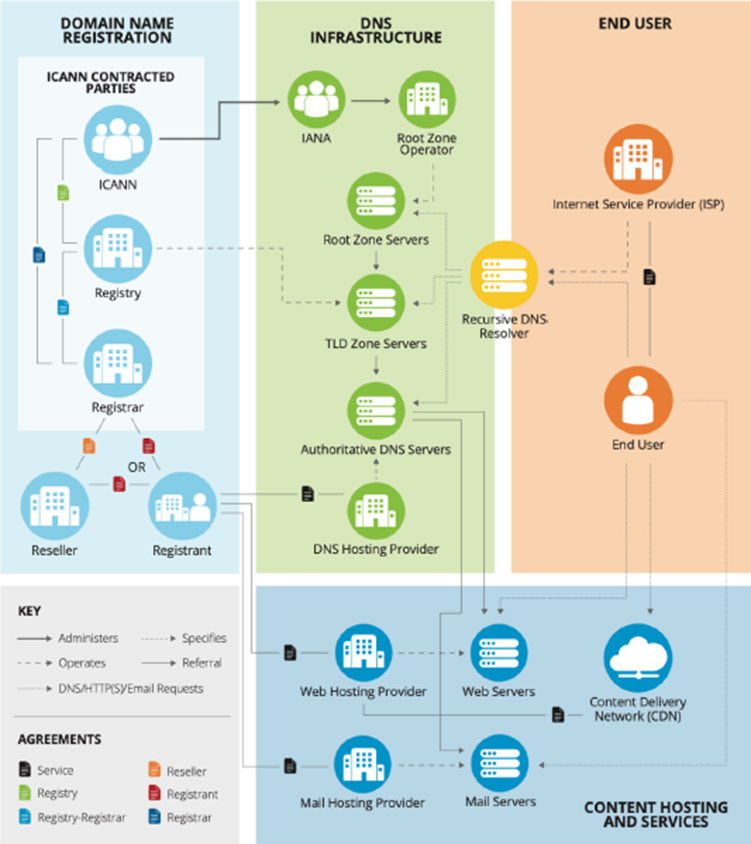
\includegraphics[width=0.9\linewidth]{background/DNSECO.png}
    \caption{DNS Ecosystem Contractually Related to ICANN (image
courtesy of Verisign and originally published in SSAC 115 adapted from \cite{SSAC2023SAC115})}
    \label{fig:fig14}
\end{figure}


\section{Technological Advancements}

The mitigation of DNS abuse is increasingly influenced by the integration of artificial intelligence (AI) and machine learning technologies \cite{goethals2021enabling}. At the helm of this evolution are innovative tools such as the iQ Domain Risk Score, which employs machine learning and string analytics to proactively detect potential domain abuses now of registration \cite{dnsabuseAI2023}. This tool aims to act as a mitigation measure by analysing domains against criteria indicative of malicious intent, thereby attempting to stop abuse before it even starts. Additionally, the field is witnessing a transformative shift in analysing abuse report evidence through the adoption of Large Language Models (LLMs), such as generative pre-trained transformers (GPTs). These models are highly adept at parsing and understanding complex data patterns that could be missed by humans, enhancing the efficiency and automation of DNS abuse mitigation efforts, and forming a more dynamic defence against cyber threats. However, this progress also highlights an emerging challenge: the potential for malicious entities to exploit AI technologies themselves \cite{halvorsenAI2023}.  Consequently, the intersection of AI and machine learning with DNS abuse mitigation not only heralds significant advancements in cybersecurity strategies, but also emphasises the need for vigilance to prevent these technologies from being used for harmful purposes. This pivotal moment in the fight against DNS abuse underscores the need for ongoing innovation and adaptation to effectively secure digital ecosystems.

\subsection{Role of AI \& ML}

The introduction of AI and machine learning technologies into DNS abuse mitigation marks the beginning of an innovative era focused on proactive detection and neutralisation of cyber threats \cite{tariq2023critical}.  This approach facilitates the rapid analysis of large datasets to uncover patterns indicative of malicious intent in DNS queries. For example, machine learning techniques have been highly effective in analysing DNS queries to classify domain names, significantly improving the detection of domains linked to malware \cite{LiMaliciousDomainDetection2020}. Furthermore, the application of neural network models, such as the Extreme Learning Machine (ELM), has achieved accuracy rates above 95\% in the identification of malicious domains, demonstrating the predictive power of AI in combating cyber threats \cite{ZouDNSGraphMining2015}. Additionally, the technique of DNS graph mining has illuminated AI's potential within cybersecurity frameworks, with methodologies like belief propagation algorithms achieving high precision in identifying infected hosts and malicious domains. These examples underscore the vital role of AI and machine learning in supporting DNS abuse, paving new avenues for early detection and swift mitigation of potential abuses. However, the complexity of AI models and the demand for transparency in their decision-making processes present ongoing challenges. Integrating AI into DNS abuse mitigation strategies improves security measures, but also requires careful attention to ethical considerations and the establishment of governance frameworks \cite{AntonakakisMalwareDomainsUpperDNS2011}. AI and machine learning can help improve DNS abuse mitigation, but experts must be clear about the problem.  It is important to understand how AI models make certain decisions. This helps build trust and ensures that people are responsible for them. There are difficulties in making things clear, such as needing to write down what data was used for training, telling others about the things that affect choices, and explaining how models change to face new risks. It is still difficult to find the right balance between the complexity needed for good threat detection and the openness needed for blame.

In summary,AI and ML are valuable in protecting against rapidly evolving cyber threats and a wide range of devices, including those in the IoT. However, their predictive accuracy can be limited by the quality and quantity of data used for training. Sophisticated attacks designed to evade detection algorithms present a notable challenge, underscoring the importance of continuous learning and adaptation in AI/ML models to maintain their effectiveness.


\section{Case Studies and Real-World Applications}

In recent years, technology has become so widespread that we have witnessed an unmatched number and complexity of cyber threats. A significant vulnerability that can be exploited is the DNS domain name system, a critical part of the internet infrastructure that translates human-readable names into IP addresses \cite{kumari2021sac115}. 

\begin{enumerate} 

\item\textbf{ Case Study 1: OilRig DNS Tunneling Attack }

The case of OilRig reflects the use of custom DNS tunnelling protocols for command and control (C2) operations, thus making it dual-use in nature, both in normal operation and on a fallback communication channel \cite{paloaltonetworks2021dnsattacks}.The xHunt campaign \cite{unit42_xhunt_2021} followed a similar trend of including Snugy backdoor implants in targets of Middle Eastern government organisations and keeping track of them using DNS tunnelling for communication with its C2.  These are examples that underscore the strategic use by adversaries of DNS tunneling techniques for stealthiness and resilience within the context of their operations \cite{unit42_2021}.

\captionsetup{font= footnotesize}
\begin{figure}[H]
    \centering
    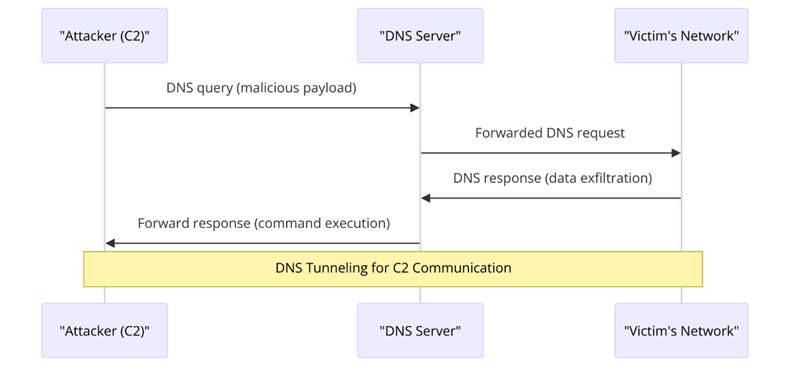
\includegraphics[width=\textwidth]{background/DNSTuu.png}
    \caption{DNS tunneling communication between the attacker's command and control (C2) infrastructure and the victim's network.}
    \label{fig:figTen}
\end{figure}



\item\textbf{ Case Study 2: SUNBURST Use of DGAs}

SUNBURST backdoor associated with the breach of the SolarWinds supply chain represents a case in which the use of DGAs is critical, if not only, to conceal communications and system details \cite{paloaltonetworks2021dnsattacks}. The SUNBURST backdoor applies the deep use of DNS manipulation for evasion purposes and subsequent attack stages by encoding basic system identifiers and the usage of DGAs for C2 check-ins \cite{unit42_solarstorm_2021}.

\captionsetup{font= footnotesize}
\begin{figure}[H] 
    \centering
    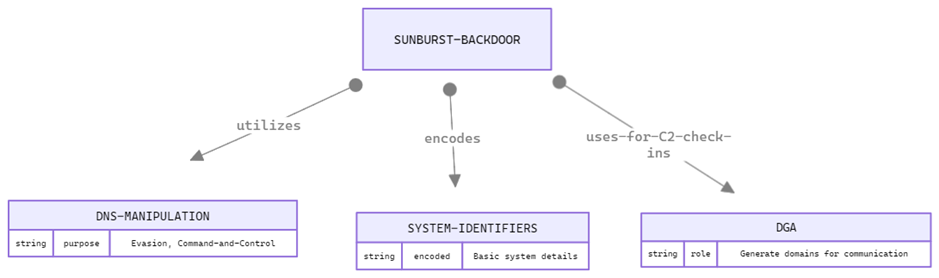
\includegraphics[width=0.8\linewidth]{background/SUNDNS.png}
    \caption{SUNBURST backdoor's utilization of DGAs and its associated components.}
    \label{fig:figEleven}
\end{figure}

\item\textbf{ Case Study 3: Fast Flux Techniques}
The presence of several C2 domains related to the Smoke Loader malware family using Fast Flux techniques only further underscores the difficulties associated with the tracking and eradication of DNS-enabled threats. \cite{paloaltonetworks2021dnsattacks}.The major takeaway in the rapid rotation of IP addresses of this method points to the dynamism of strategies used in malicious communications, thus improving the means of defence by cybersecurity \cite{unit42_fastflux_2021}.

\captionsetup{font= footnotesize}
\begin{figure}[H]
    \centering
    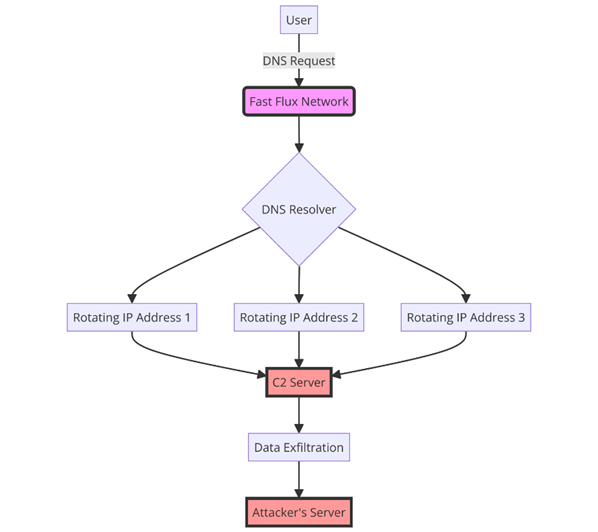
\includegraphics[width=0.8\linewidth]{background/FastFluDNS.png}
    \caption{The usage of Fast Flux techniques by the Smoke Loader malware family for dynamic C2 domain communications.}
    \label{fig:figTweleve}
\end{figure}


\item\textbf{Case Study 4:  Malicious Newly Registered Domains (NRDs)}

Malicious NRDs crafted opportunistically in the context of the pandemic expose how threat actors exploit current events to engineer targeted attacks. \cite{paloaltonetworks2021dnsattacks} From domains that mirror the information resources of COVID-19 to those that feign government relief programmes, the evolution of such attacks reflects a calculated approach to exploiting public interest and vulnerabilities  \cite{unit42_covid19_phishing_2021} .

\captionsetup{font= footnotesize}
\begin{figure}[H]
    \centering
    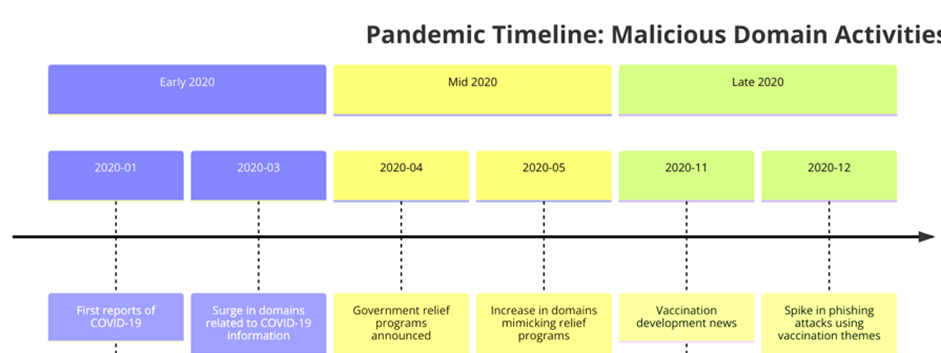
\includegraphics[width=0.8\linewidth]{background/PandemicTime.png}
    \caption{The usage of Fast Flux techniques by the Smoke Loader malware family for dynamic C2 domain communications.}
    \label{fig:figThirteen}
\end{figure}

\end{enumerate}

In the coronavirus pandemic, too, phishing attacks changed to initially targeting PPE and testing kits, then turning to government stimulus programmes and subsequently enlisting vaccine distribution. Several of them, in fact, employed sophisticated tools, such as MFA pretending as the US Federal Trade Commission and brands such as Pfizer and BioNTech, to steal credentials. where it emphasised that there was a 530\% surge in vaccine-related phishing attempts and a 189\% increase in attacks on pharmacies and hospitals from December last year to February this year. Advice was given to individuals and organisations that includes being cautious in email and website transactions, advancing security awareness training, and adopting multifactor authentication.

Since January 2020, a total of 69,950 COVID-19 related phishing URLs have been received, of which 33,447 are specifically dedicated to COVID-19. The data have been normalised in such a way that the peak of each topic is at 100\%. The results showed much steadier phishing when it came to topics such as pharmaceuticals and virtual meeting platforms (e.g., Zoom) with vaccines and testing showing sharper rises and falls in the attention of scammers.

\captionsetup{font= footnotesize}
\begin{figure}[H]
    \centering
    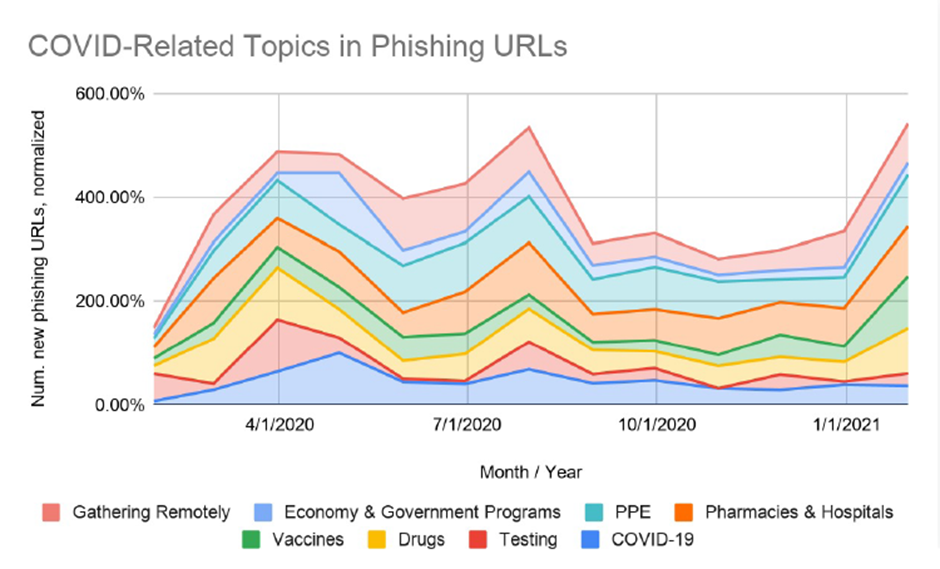
\includegraphics[width=0.8\linewidth]{background/CovidPhising.png}
    \caption{Development trends in the majority of COVID-19-related phishing content hosting sites during the period from January 2020 to February 2021. Adapted from \cite{Unit42AtricleCovidPhishing2021}.}
    \label{fig:figFourteen}
\end{figure}

It is evident that a large portion of COVID-19 themed phishing pages targeted leading brands for phishing business credentials, such as Microsoft login, Webmail, and Outlook login. For example, about 23\% of these phishing URLs were posed as Microsoft login pages. This threat has particularly highlighted the shift towards remote work in the pandemic, and hence magnified the relevance of these attacks as one of the foremost methods that bad actors are taking on.


\captionsetup{font= footnotesize}
\begin{figure}[H]
    \centering
    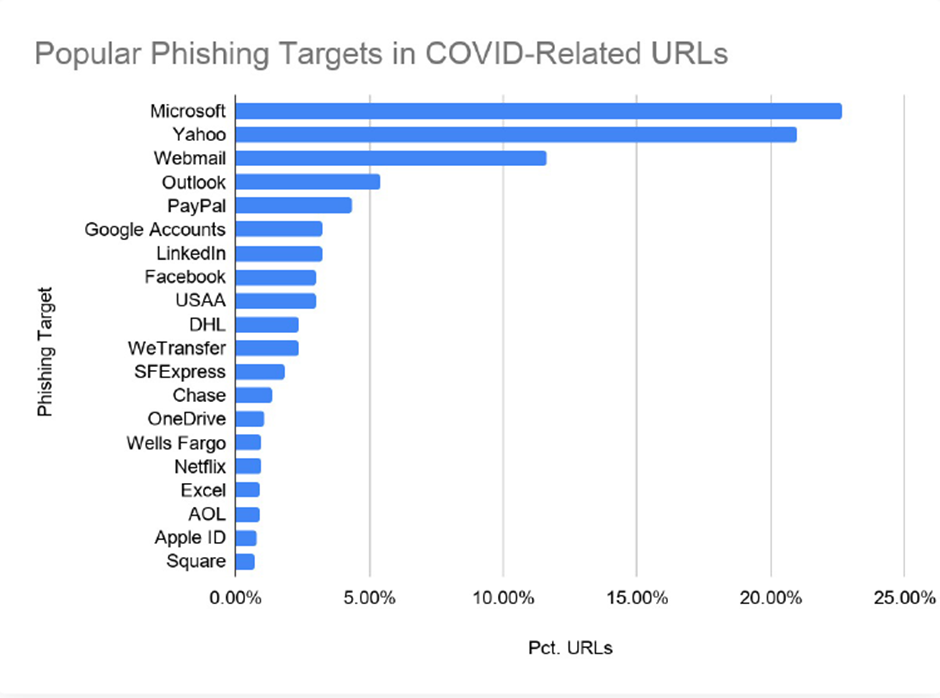
\includegraphics[width=0.8\linewidth]{background/TOPCOVIDURLS.png}
    \caption{Top spoofed websites in COVID-themed phishing attacks (global), where the percentage in each column is the percentage of phishing volume per site and category. Adapted from \cite{Unit42AtricleCovidPhishing2021}.}
    \label{fig:figFiveteen}
\end{figure}

Thus, this clearly indicates a situation whereby the attackers set up websites frequently for COVID-19 themed phishing attacks. Many of these phishing pages are found on sites created less than 32 days, meaning that these sites are launched with specific purposes in view of these imminent attacks. The strategy allows attackers to customise their messages and URLs to the current pandemic trends, indicating the dynamism behind such cyber threats.

\captionsetup{font= footnotesize}
\begin{figure}[H]
    \centering
    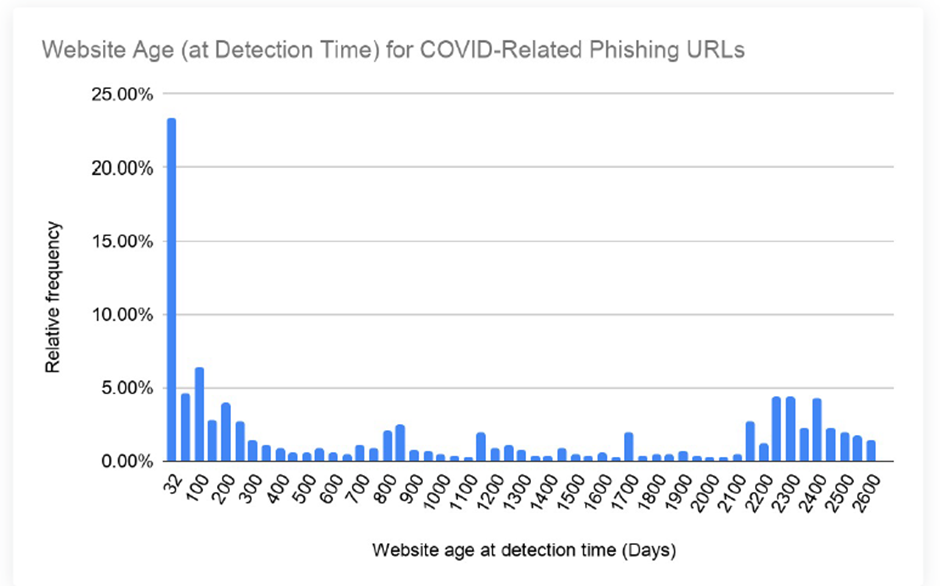
\includegraphics[width=0.8\linewidth]{background/AgeCovid.png}
    \caption{Statistic of lifespan distribution of COVID-19-related phishing content hosting sites when the sites are reported. Adapted from \cite{Unit42AtricleCovidPhishing2021}.}
    \label{fig:figSixteen}
\end{figure}


\section{Challenges \& Future Directions}

Mitigating DNS abuse demands an immediate stop to the rapid evolution of cyber threats, underscoring the critical need for rapid global cooperation and the implementation of advanced technology. The key challenge is to achieve a fine balance between reducing false positives and accurately identifying genuine threats, while simultaneously advancing beyond the limitations of outdated technologies \cite{pour2023comprehensive}. The future of this domain largely depends on researchers' ability to enhance technological solutions, particularly focussing on the improvement of AI algorithms for deeper analysis of DNS traffic patterns. This opens a promising pathway for the creation and application of locally developed tools, providing innovative strategies to strengthen DNS defences. The ability to navigate the complex landscape of DNS abuse will require stakeholders to be agile in responding to emerging threats and developing novel solutions. The collective push towards the evolution of technology and methodologies will play a pivotal role in shaping effective DNS abuse management strategies in the years ahead.


\subsection{Identification of Current Challenges}

Mitigating DNS abuse involves developing strategies that should not only be proactive, but kept constantly up to date to handle the changing environment of cyber threats. The fluid nature of these threats means updating current protocols as well as developing new defence methods. With bad actors constantly reviewing their methods to take advantage of the vulnerability of DNS, it has become imperative that the cybersecurity industry continuously updates its defence mechanisms \cite{bhattacharya2023dns}. Being a global phenomenon, the Internet and hence DNS abuse being transnational in character, there is no other alternative than international cooperation. The effectiveness of DNS abuse management would be based on collaborative work across national borders, where experts in different geographical areas come together to share their knowledge and resources \cite{altulaihan2022cybersecurity}. The legal and regulatory framework varies in the various jurisdictions, making it difficult to reach a consensus on the regulations, standards, and enforcement actions. Another big challenge is that, to mitigate DNS abuse, the requirement is necessary to eliminate both false positives and negatives. Balance must be established in such a way that rather strict measures may reduce user experience, while, at the same time, being liberal might bring less detection of malicious activities. The cybersecurity community must continue to advance its detection and response capabilities, due to the increasing levels of sophistication used by DNS abusers. This will keep the security and integrity of the DNS system in good shape, thus protecting this vital part of the Internet infrastructure.

\subsection{Discussion on Future Research Directions and Technologies}

At the ICANN77 meeting, developments on mitigating DNS abuse were presented. These included the draughting of changes mandating that registrars and registries respond to abuse notifications, which contributed to a decline in global abuse levels after Freenom's legal response. Although the ccNSO Domain Abuse Steering Committee argued for a proactive mitigation strategy, the gNSO's analysis found minimal abuse rates in EU ccTLDs, which it attributed to market maturity and non-profit models \cite{VanRoste2023}. To improve domain security and enable international cooperation against changing cyberthreats, future initiatives will focus on creating cutting-edge tools and using technologies such as artificial intelligence and machine learning. This means that we need to look at more complex AI and machine learning tools that can understand the details of web traffic, which will make the results more accurate and stop the sending of wrong signals \cite{ISG2023}.

\section{Summary of Findings}

Research on the transparency of DNS abuse mitigation emphasises how threats are always changing and how mitigation techniques must evolve as well. It highlights how important community involvement and transparency are to fostering trust. Although technological advancements, especially in AI and machine learning, are essential for threat detection, their implementation must be carefully considered. Practical examples provide insight into the efficacy of various strategies. Maintaining a balance between new mitigation measures and effective teamwork and communication is a constant issue. To effectively address DNS abuse, future efforts should focus on using technology, international cooperation, and standardised information exchange.






















